OSS possiede una propria base di dati formata da 19 tabelle e 5 viste. Si vogliono mantenere logicamente separati i dati relativi alla PadovaCard.\\

Di seguito venogno riportati lo schema concettuale, lo schema logico e il DDL dell'espansione del database, mentre non viene riportata la struttura del database esistente in quanto non interagirà con le nuove tabelle.\\

Una nota sui nomi delle tabelle è d'obbligo, CackePHP richiede l'utilizzo di una sintassi standard per i nomi delle tabelle, necessaria per effettuare l'accoppiamento model-tabella. Risulta quindi necessario utilizzare nomi inglesi plurali o nomi italiani che terminano per s.
\subsubsection{Modello concettuale}
\begin{figure}[H]
\centering
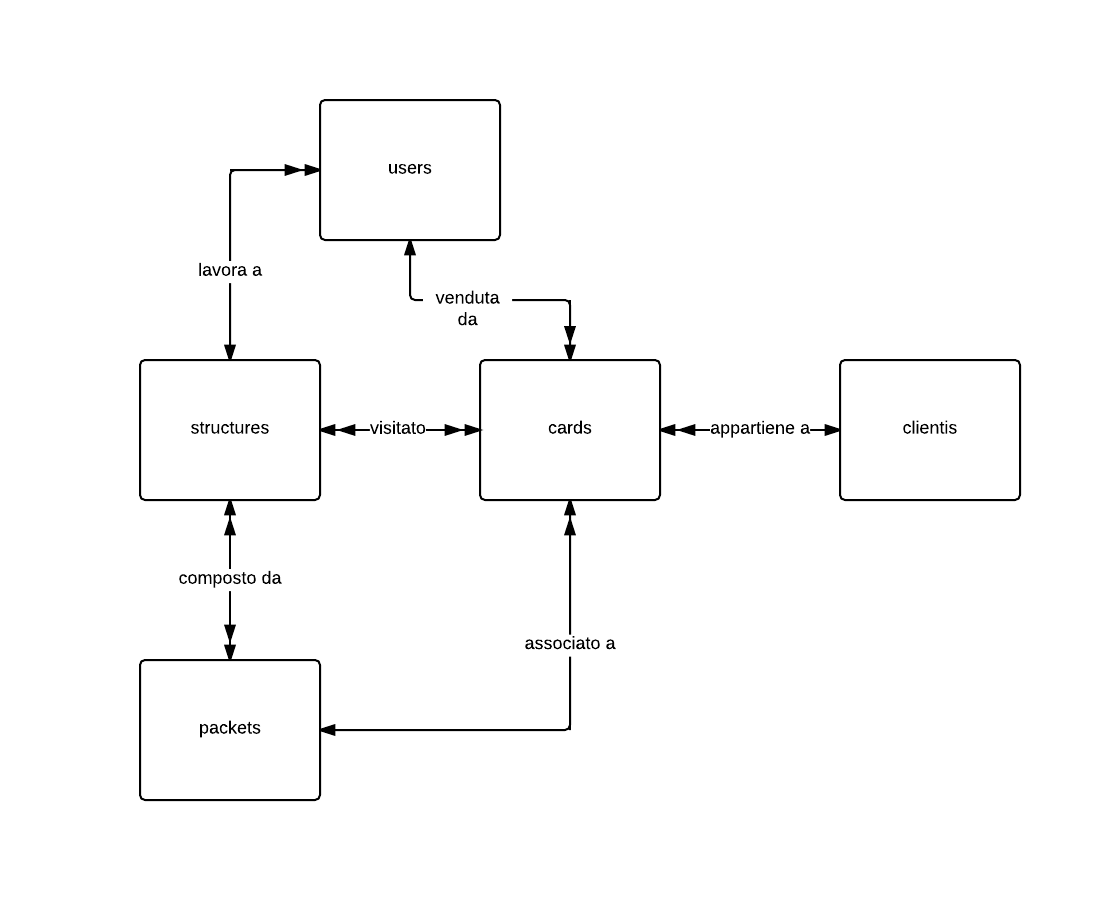
\includegraphics[width=1\textwidth]{images/concettuale.png}
\caption{Modello concettuale della base di dati}
\end{figure}
L'espansione del database già esistente si compone di 3 tabelle, cards, packets e structures mentre clientis e users sono già presenti.
Le nuove tabelle saranno collegate al database esistente tramite clientis e users utilizzando chiavi esterne.\\ \\
\textbf{Tabelle}
\begin{itemize}
\item \textbf{card:} contiene tutte le informazioni sulle PadovaCard;
\item \textbf{clientis:} contiene l'anagrafica degli utenti che hanno acquistato una PadovaCard o altri articoli che necessitano di anagrafica dal sistema;
\item \textbf{packets:} contiene i dati relativi ai pacchetti associabili alla PadovaCard. Ricordiamo che un pacchetto è un insieme di strutture visitabili;
\item \textbf{structures:} contiene i dati su tutte le strutture convenzionate con PadovaCard;
\item \textbf{users:} contiene i dati relativi agli operatori e al personale delle strutture. In futuro potrebbe contenere anche quelli relativi agli hotel.
\end{itemize}
\textbf{Relazioni}
\begin{itemize}
\item \textbf{appartiene a:} cards è connessa con una relazione uno a molti a clientis perchè ogni utente può avere una sola PadovaCard attiva, ma più di una non attive, ogni Padovacard attiva deve essere connessa ad un cliente, mentre quelle inattive possono non esserlo. Questa distinzione si rende necessaria per quando in futuro gli utenti potranno acquistare via web le PadovaCard. Ci sarà un periodo di tempo tra la creazione della carta e l'inserimento di tutti i nominativi a causa degli ordini di più PadovaCard. Escludendo questo requisito anche le PadovaCard inattive hanno un nominativo associato
\item \textbf{associata a:} cards è connessa con una relazione uno a molti a packets perchè ad ogni PadovaCard è associato un solo pacchetto di strutture, mentre un pacchetto può essere associato a più Padovacard;
\item \textbf{composto da:} packets è collegato con una relazione molti a molti a structures in quanto ogni pacchetto è formato da più strutture ed ogni struttura può essere presente su più pacchetti;
\item \textbf{lavora a:} users è collegato con una relazione uno a molti a strcutures per mantenere i dati relativi al personale delle strutture;
\item \textbf{venduta da:} cards è connessa con una relazione uno a molti ad users in quanto bisogna tener traccia di quale operatore vende una PadovaCard, una Padovacard può essere venduta da un solo operatore e un operatore può vendere più PadovaCard. Una carta può non essere venduta da un operatore, nel caso in cui l'acquisto sia fatto via internet;
\item \textbf{visitato:} cards è connesso con una relazione molti a molti a strutture perchè è necessario tener traccia di quali struttre ha visitato l'utente per impedire che con la stessa PadovaCard venga visitata più volte la stessa struttura.


\end{itemize}


\subsubsection{Modello logico-relazionale}\label{logicorelazionale}

\begin{figure}[H]
\centering
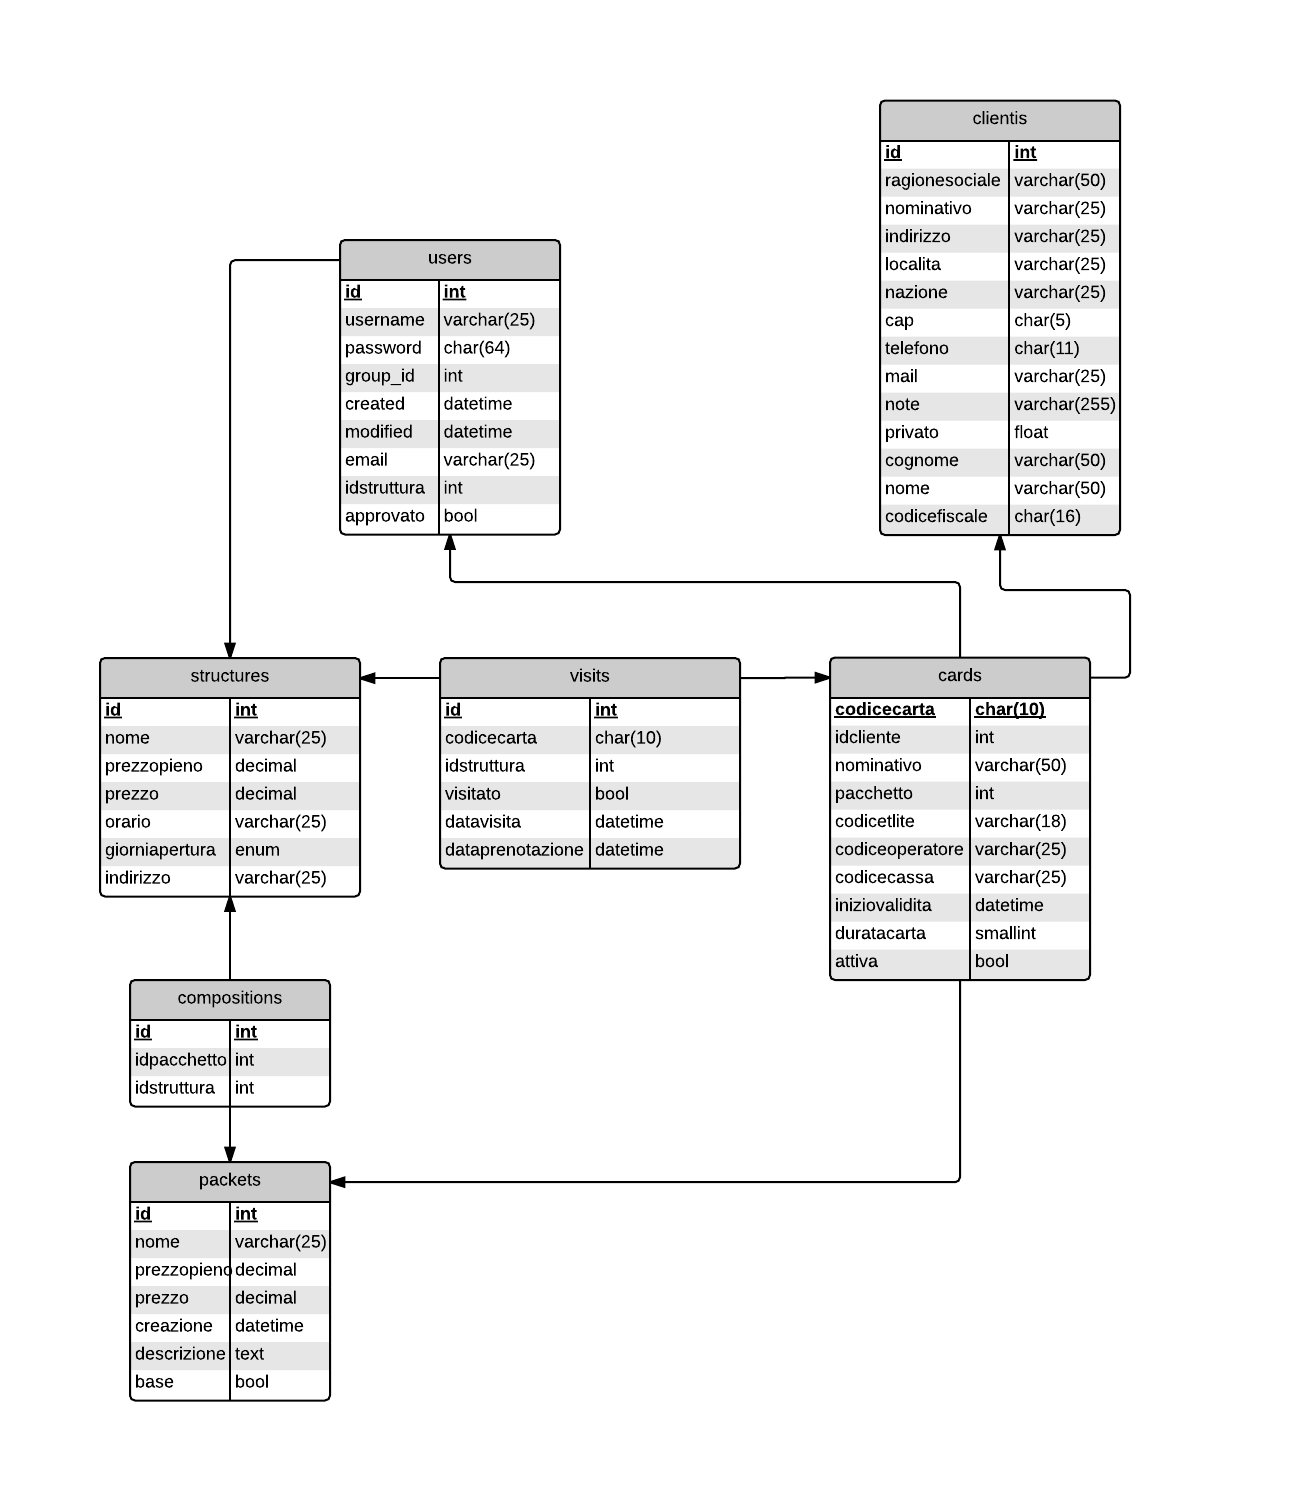
\includegraphics[width=1\textwidth]{images/logico.png}
\caption{Modello logico della base di dati}
\end{figure}
CakePHP prevede che ogni tabella abbia una sola chiave primaria in quanto non supporta chiavi primarie composite, per questo è necessario aggiungere una chiave primaria "di servizio" per CakePHP in tabelle come visite e composizione.\\ \\
\textbf{Note di progettazione}\\ \\
Inizialmente cards conteneva un campo dal nome prenotazionecappella, di tipo datetime, che doveva contenere la data e l'ora della prenotazione alla \cappella. \'E stato deciso di spostare tale campo sulla tabella visits e rinominarlo dataprenotazione. Questo permette di gestire la prenotazione a più strutture nel caso in cui in futuro ci sia tale necessità. \'E altresi vero che la maggior parte dei record avrà Null come valore di dataprenotazione, ma essendo questo di tipo datetime si è stimato uno spreco di memoria nel caso peggiore di meno di 3 Megabyte annui. Il calcolo è il seguente:
Dimensione di datetime $*$ numero stimato di PadovaCard vendute in un anno $*$ numero massimo di strutture per pacchetto = $8byte*20000*15 $. \\

Attualmente per le password vengono usati campi di tipo char(40) ovvero un campo che può contenere fino ad un massimo di 40 caratteri, sufficienti a contenere l'output della funziona hash \glossario{MD5}. Il tirocinante propone di utilizzare un campo char(64) in previsione dell'utilizzo dell'hash \glossario{SHA256}. Tale cambio è motivato nella Sezione \ref{hash}. \\

Nella tabella users è presente un campo username di tipo varchar(255). Nonostante varchar occupi solamente lo spazio per i caratteri effettivamente scritti, quando vengono create le tabelle temporanee durante le query viene allocata la lunghezza massima. Per questo il tirocinante propone di modificare varchar(255) in varchar(25), più che sufficiente per i valori di tale campo. \\

Clientis contiene i campi cap, telefono e note di tipo varchar(25). Il tirocinante propone di modificare il tipo di cap in char(5), telefono in char(11) e note in varchar(255) in quanto tale valore per varchar è il massimo ottenibile con un solo byte di overhead. Codicefiscale che ora ha tipo varchar(16) viene modificato in tipo char(16). \\

La chiave primaria di cards è codicecarta, con tipo char(10). Si è scelto di utilizzare codicecarta e non un id auto increment in quanto è univoca e permette di evitare una join durante la lettura di visits. Questo è ottimale in quanto visits sarà la tabella con più query in lettura, mentre si stima la perdita di efficienza nell'uso di char invece di int inferiore al 20\% nel caso peggiore, considerando la lunghezza del char, il fatto che è indicizzato e che il motore usato è \glossario{INNODB}. \\

Sempre in cards duratacarta è uno samllint. Ad oggi sono previste solo due durate, 48 e 72 ore, per cui un tipo bool sarebbe stato sufficiente ma uno smallint permette di creare più di due tipologie di durata. \\

La tabella packets contiene il campo descrizione di tipo text, ritenuto necessario se si vuole salvare qui la descrizione completa della struttura che apparirà nel sito che l'utente adrà a consultare per ottenere le informazioni sulla PadovaCard. \\

Cards contiene il flag attiva che indica se la carta è stata pagata, e se è quindi valida. Questo flag è settato subito a 1 se il pagamento avviene con contanti o carta di credito, mentre viene posto a 0 in attesa del pagamento con bonifico. \\

Cards contiene un campo nominativo e un campo idcliente. Idcliente viene utilizzato per collegare la PadovaCard all'anagrafica di chi ha effettuato l'ordine, che può essere una persona sia fisica che giuridica. Nominativo contiene il nome del proprietario della PadovaCard e sarà il nome presente nel voucher. Per questo motivo ci potranno essere più PadovaCard attive con lo stesso idcliente mentre il nominativo sarà unico.\\

Per i campi che rappresentano denaro è stato utilizzato il tipo decimal e si è deciso di continuare ad utilizzarlo in quanto non presenta rischi di approssimazione che invece ha il tipo float. \\ \\
\textbf{Tabelle}\\ \\
Nella seguente Sezione verranno descritte nel dettaglio le tabelle che saranno create. Per ogni tabella è fornita una descrizione sul contenuto e un elenco dei suoi campi, comprensivo di tipo e altre note. \\ \\
PK indica che tale campo è \glossario{chiave primaria} della tabella. \\
FK indica che tale campo  è \glossario{chiave esterna} della tabella.\\
\\ \\
CARDS: Contiene tutti i dati relativi alla PadovaCard.
\begin{itemize}
\item codicecarta: varchar(10) \textit{\textless PK\textgreater}
\item idcliente: int \textit{\textless FK\textgreater}
\item pacchetto: int \textit{\textless FK\textgreater}
\item nominativo: varchar(50)
\item codicetlite: varchar(18)
\item codiceopertatore: varchar(25)
\item codicecassa: varchar(25)
\item iniziovalidita: datetime
\item duratacarta: smallint
\item attiva: bool 
\end{itemize}
CLIENTIS: Contiene l'anagrafice degli utenti.
\begin{itemize}
\item id: int \textit{\textless PK\textgreater}
\item ragionesociale: varchar(50)
\item nominativo: varchar(25)
\item indirizzo: varchar(25)
\item localita: varchar(25)
\item nazione: varchar(25)
\item cap: char(5)
\item telefono: char(11)
\item mail: varchar(25)
\item note: varchar(255)
\item privato: float
\item cognome: varchar(50)
\item nome: varchar(50)
\item codicefiscale: char(16)
\end{itemize}
COMPOSITIONS: Tabella creata dalla relazione "composta da", collega le strutture ai pacchetti.
\begin{itemize}
\item id: int \textit{\textless PK\textgreater}
\item idpacchetto: int \textit{\textless FK\textgreater}
\item idstruttura: int \textit{\textless FK\textgreater}
\end{itemize}
PACKETS: Contiene i dati relativi ai pacchetti, composizioni di strutture visitabili.
\begin{itemize}
\item id: int \textit{\textless PK\textgreater}
\item nome: varchar(25)
\item prezzopieno: decimal
\item prezzo: decimal
\item creazione: datetime
\item descrizione: text
\item base: bool
\end{itemize}
STRUCTURES: Contiene i dati relativi alle strutture convenzionate con PadovaCard.
\begin{itemize}
\item id: int \textit{\textless PK\textgreater}
\item nome: varchar(25)
\item prezzopieno: decimal
\item prezzo: decimal
\item orario: datetime
\item giorniapertura: enum('LU','MA','ME','GI','VE','SA','DO')
\item indirizzo: varchar(25)
\end{itemize}
USERS: Contiene i dati riguardanti gli operatori e il personale delle strutture.
\begin{itemize}
\item id: int \textit{\textless PK\textgreater}
\item username: varchar(25)
\item password: char(64)
\item group\_id: int
\item created: datetime
\item modified: datetime
\item email: varchar(25)
\item idstruttura int \textit{\textless FK\textgreater}
\item approvato: bool
\end{itemize}
VISITS: Tabella creata dalla relazione "visitato", tiene traccia di quali strutture sono state visitate da una data PadovaCard, e di eventuali prenotazioni.
\begin{itemize}
\item id INT \textit{\textless PK\textgreater}
\item codicecarta: varchar(10) \textit{\textless FK\textgreater}
\item idstruttura: int \textit{\textless FK\textgreater}
\item visitato: bool
\item datavisita: datetime
\item dataprenotazione: datetime
\end{itemize}
\textbf{Definizione dello schema logico tramite \glossario{DDL} di MySQL}
\lstset{frame=single}
\begin{center}
\begin{lstlisting}
create table clientis (
  id int(11) not null auto_increment,
  ragionesociale varchar(50) default null,
  nominativo varchar(25) default null,
  indirizzo varchar(25) default null,
  localita varchar(25) default null,
  nazione varchar(25) default null,
  cap varchar(25) default null,
  telefono varchar(25) default null,
  mail varchar(50) default null,
  note varchar(25) default null,
  privato float default null,
  cognome varchar(50) default null,
  nome varchar(50) default null,
  codfiscale varchar(16) default null,
  primary key (id)
) ENGINE=InnoDB  DEFAULT CHARSET=utf8 AUTO_INCREMENT=585;

alter table clientis 
	modify column cap char(5),
    modify column telefono char(11),
    modify column note varchar(255);

create table users (
  id int(11) NOT NULL auto_increment,
  username varchar(255) not null,
  password char(40) not null,
  group_id int(11) not null,
  created datetime default null,
  modified datetime default null,
  PRIMARY KEY  (id)
) ENGINE=InnoDB  DEFAULT CHARSET=utf8 AUTO_INCREMENT=51;

alter table users
	modify column password char(64);
    modify column username varchar(25),
    add email varchar(25),
    add approvato bool,
    add idstruttura int,
    add foreign key (idstruttura) references structures (id);

create table packets(
	id int not null auto_increment,
	nome varchar(25) not null,
    prezzopieno decimal default null,
    prezzo decimal default null,
    creazione datetime default null,
	descrizione text default null,
    base bool default 0,
	primary key (id)
)ENGINE=InnoDB DEFAULT CHARSET=utf8; 
	
create table structures(
	id int not null auto_increment,
    nome varchar(25) not null,
    prezzopieno decimal default null,
    prezzo decimal default null,
    orario varchar(25) default null,
    giorniapertura enum('LU','MA','ME','GI','VE','SA','DO') default null,
    indirizzo varchar(25) default null,
	primary key (id)
)ENGINE=InnoDB DEFAULT CHARSET=utf8;

create table compositions(
	id int not null auto_increment,
    idpacchetto int not null,
    idstruttura int not null,
    primary key (id),
    foreign key (idpacchetto) references packets(id),
    foreign key (idstruttura) references structures(id)
)ENGINE=InnoDB DEFAULT CHARSET=utf8;

create table cards(
codicecarta char(10) not null,
idcliente int not null,
pacchetto int not null,
nominativo varchar(50),
codicetlite varchar(18) not null,
codiceoperatore varchar(25),
codicecassa varchar(25),
iniziovalidita datetime,
duratacarta smallint not null,
attiva bool default 0,
foreign key (idcliente) references clientis(id),
foreign key (pacchetto) references packets(id),
primary key (codicecarta)
)ENGINE=InnoDB DEFAULT CHARSET=utf8;
\end{lstlisting}
\end{center}